%%%%%%%%%%%%%%%%%%%%%%%%%%%%%%%%%%%%%%%%%
% Journal Article
% LaTeX Template
% Version 1.3 (9/9/13)
%
% This template has been downloaded from:
% http://www.LaTeXTemplates.com
%
% Original author:
% Frits Wenneker (http://www.howtotex.com)
%
% License:
% CC BY-NC-SA 3.0 (http://creativecommons.org/licenses/by-nc-sa/3.0/)
%
%%%%%%%%%%%%%%%%%%%%%%%%%%%%%%%%%%%%%%%%%

%----------------------------------------------------------------------------------------
%	PACKAGES AND OTHER DOCUMENT CONFIGURATIONS
%----------------------------------------------------------------------------------------

\documentclass[twocolumn]{article}

%% Load graphicx package
\usepackage{graphicx}
%\usepackage[font=small]{subfig}
\graphicspath{{images/}}
\DeclareGraphicsExtensions{.pdf,.png,.jpg}
%\usepackage{amsmath}
\usepackage[font=small]{subfig}

\usepackage{lipsum} % Package to generate dummy text throughout this template

\usepackage[sc]{mathpazo} % Use the Palatino font
\usepackage[T1]{fontenc} % Use 8-bit encoding that has 256 glyphs
\linespread{1.05} % Line spacing - Palatino needs more space between lines
\usepackage{microtype} % Slightly tweak font spacing for aesthetics

\usepackage[hmarginratio=1:1,top=32mm,columnsep=20pt]{geometry} % Document margins
%\usepackage{multicol} % Used for the two-column layout of the document
\usepackage[hang, small,labelfont=bf,up,textfont=it,up]{caption} % Custom captions under/above floats in tables or figures
\usepackage{booktabs} % Horizontal rules in tables
\usepackage{float} % Required for tables and figures in the multi-column environment - they need to be placed in specific locations with the [H] (e.g. \begin{table}[H])
\usepackage{hyperref} % For hyperlinks in the PDF

\usepackage{lettrine} % The lettrine is the first enlarged letter at the beginning of the text
\usepackage{paralist} % Used for the compactitem environment which makes bullet points with less space between them

\usepackage{abstract} % Allows abstract customization
\renewcommand{\abstractnamefont}{\normalfont\bfseries} % Set the "Abstract" text to bold
\renewcommand{\abstracttextfont}{\normalfont\small\itshape} % Set the abstract itself to small italic text

\usepackage{titlesec} % Allows customization of titles
\renewcommand\thesection{\Roman{section}} % Roman numerals for the sections
\renewcommand\thesubsection{\Roman{subsection}} % Roman numerals for subsections
\titleformat{\section}[block]{\large\scshape\centering}{\thesection.}{1em}{} % Change the look of the section titles
\titleformat{\subsection}[block]{\large}{\thesubsection.}{1em}{} % Change the look of the section titles

\usepackage{fancyhdr} % Headers and footers
\pagestyle{fancy} % All pages have headers and footers
\fancyhead{} % Blank out the default header
\fancyfoot{} % Blank out the default footer
\fancyhead[C]{European Wind Energy Association Conference  $\bullet$ March 2014 $\bullet$ Barcelona, Spain} % Custom header text
\fancyfoot[RO,LE]{\thepage} % Custom footer text

%----------------------------------------------------------------------------------------
%	TITLE SECTION
%----------------------------------------------------------------------------------------

\title{\vspace{-15mm}\fontsize{24pt}{10pt}\selectfont\textbf{Sizing of Electrical Generators for Combined Wind and Wave Energy Platforms}} % Article title

\author{
\large
\textsc{Ozan Keysan, Markus A. Mueller}\thanks{Institute of Energy Systems, University of Edinburgh}\\[2mm] % Your name
\normalsize Institute of Energy Systems, University of Edinburgh \\ % Your institution
\normalsize \href{mailto:o.keysan@ed.ac.uk}{o.keysan@ed.ac.uk} % Your email address
\vspace{-5mm}
}
\date{}

%----------------------------------------------------------------------------------------

\begin{document}

\twocolumn[
\begin{@twocolumnfalse}

\maketitle % Insert title

%\thispagestyle{fancy} % All pages have headers and footers


\begin{abstract}

dggfd dgdfhfdh ghdfhdf sdgert sghdf ddsg g rrgfd fd dfe r  % Dummy abstract text

\end{abstract}

\end{@twocolumnfalse}
]
%\begin{multicols}{2} % Two-column layout throughout the main article text

\section{Introduction}

Offshore energy converters can help to utilize energy resources that remained untapped so far. Offshore wind turbines benefit from regular wind regimes and higher wind speeds. The average offshore wind speed is around 8.6 m/s, almost double of the average onshore wind speed, which is 4.6 m/s \cite{Hau2013}. Offshore energy platforms can also use wave energy to maximise electricity generation and have smoother power output. 

MARINA Platform is an EU FP7 project that aims to design combined floating wind and wave energy platforms \cite{marinaweb}. The project evaluated various combined wind and wave energy platforms in terms of manufacturability, cost of energy, reliability etc. 

One of the concepts is a floating platform that consists of a 5 MW wind turbine and 20 oscillating water columns (OWC), each with a maximum rating of 500 kW \cite{Sullivan2013} (see Fig. \ref{owc_array}).  

  \begin{figure}
    \centering
    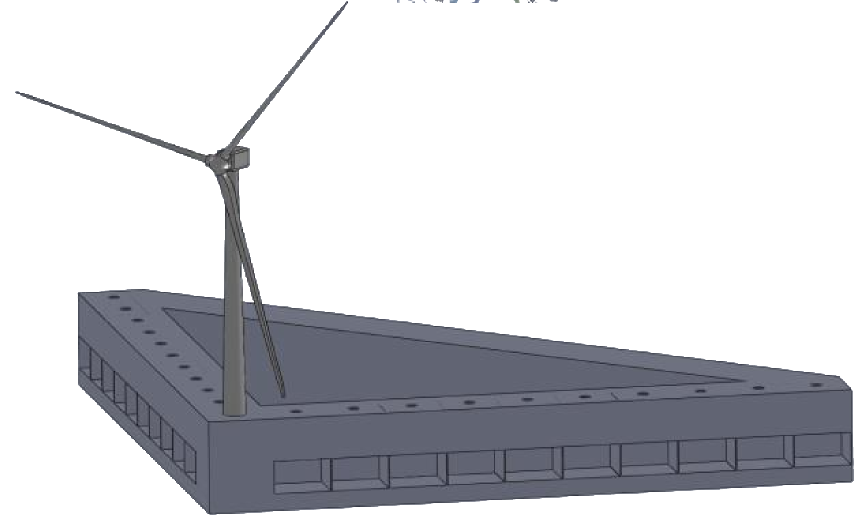
\includegraphics[]{owc_array}
    \caption{Floating OWC array with single wind turbine concept \cite{Sullivan2013}.} 
    \label{owc_array}
  \end{figure}

The power take-off system in the OWC consists of a Well's turbine, a symmetrical turbine which rotates in the same direction regardless of the direction of flow. The Well's turbine is connected to a rotary generator. For simulations a squirrel cage induction generator, directly coupled to the Well's turbine, is used. The Well's turbines usually don't have any pitch control mechanism, thus the output power is directly related the the air speed in the OWC chamber.

%------------------------------------------------

\section{Generator Type}

Induction generator is thought to be most suitable generator or OWCs. Squirrel cage induction machines (SCIG) have simple and robust structure, which makes them suitable for a wave energy converter of a floating OWC platform, where access to platform is limited by weather and sea conditions and a repair in the chamber room is not an easy task. 
The most suitable SCIG type for floating offshore platforms are marine motors, which are widely used in ships. In particular, motors used on deck have very similar operating conditions with electrical generators of OWCs. They also operate in humid and saline environment with occasional water sprays and flooding. Also in a floating platform, there is continuous rolling motion and variable temperature range similar to ships. Marine induction machines can be manufactured  with cast iron frames to reduce corrosion, can be painted with special paints or can have higher level of insulation (IP56 or IP65). 

\section{Generator Sizing}

In order to determine the optimum size of the generators, resource data measured by MARINA Platform Project work package 2 \& 4 are used. Two sites were chosen because of high wind and wave energy resource: site \#3 (off the coast of Portugal and Spain) and site \#14 (off the coast of Norway). The main specifications of the sites are presented in Table \ref{site_spec}.


\begin{table}
  \centering
  \begin{tabular}{lll}
   Parameter & Site \#3 \\
  \hline
Av. Wind Speed & 6.98 m/s \\
Av. Wave Power & 42.7 kW/m \\
Av. Wave Period & 11.84 s \\
Significant wave & 10.2 m  \\
(50-year) \\
\hline
  \end{tabular}
  \caption{Specifications of the selected sites for the OWC array \cite{Gao2012}.}
  \label{site_spec}
\end{table}


\begin{figure}[]
  \centering
  \subfloat[Significant wave height distribution.]{\label{generator_inertia}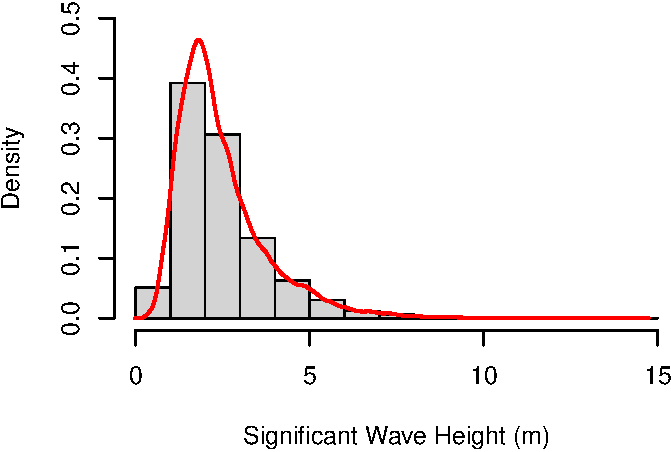
\includegraphics[width=0.45\textwidth]{spain_significant_wave}}

  \subfloat[Mean swell period distribution.]{\label{time_constant}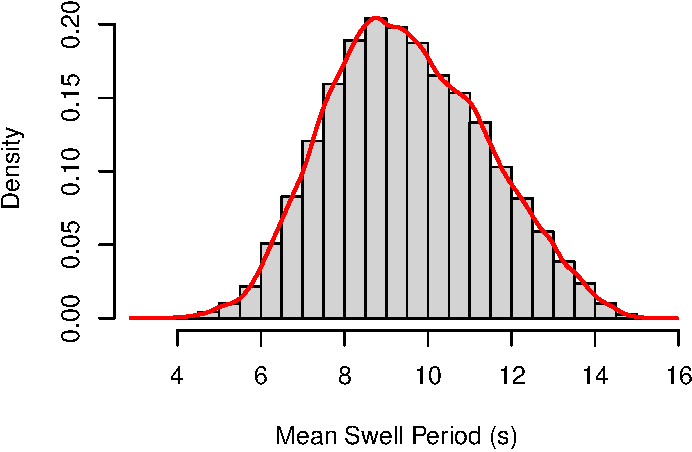
\includegraphics[width=0.45\textwidth]{spain_mean_swell}}
    \caption{Probability distribution for the wave characteristics of site \#3 (2001-2010).} 
    \label{spain_site}
\end{figure}



  \begin{figure}
    \centering
    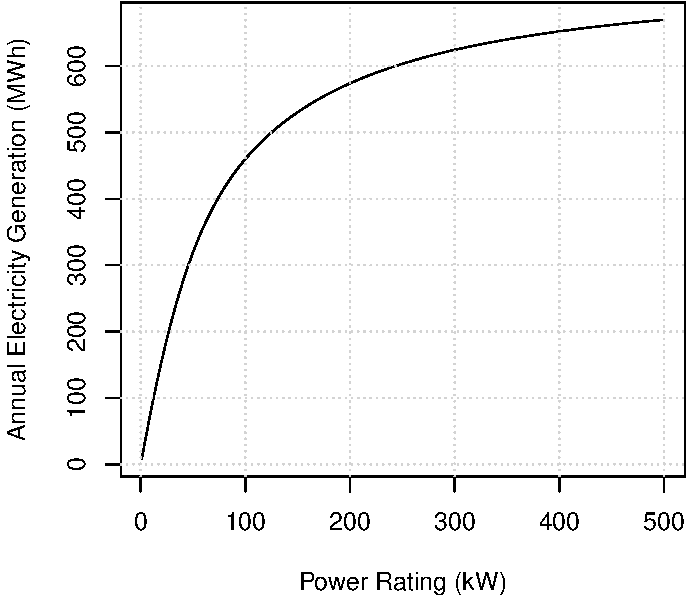
\includegraphics[width=0.5\textwidth]{generator_rating}
    \caption{Floating OWC array with single wind turbine concept } 
    \label{generator_rating}
  \end{figure}

\section{Defining Generator Parameters}

A Simulink model is developed to simulate the combined wind and wave energy platforms. Different power aggregation methods are possible and these will be presented in a different paper.

In order to evaluate the performance of different power rated machines, an accurate analytical model of electrical machine is required. The electrical machines can be represented using the equivalent electric circuit presented in Fig. \ref{equivalent_circuit}. In the circuit $R_s, R_r$ are the stator and rotor resistance, $L_{ls}, L_{lr}$ are the stator and rotor leakage inductance, $L_m$ is the magnetising inductance.


  \begin{figure}
    \centering
    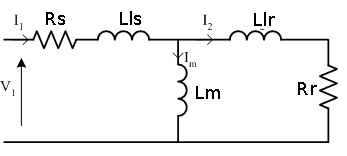
\includegraphics[width=0.45\textwidth]{equivalent_circuit}
    \caption{Equivalent circuit of an induction machine.} 
    \label{equivalent_circuit}
  \end{figure}


\subsection{Rotor Inertia}
In order to model the OWC generator, the inertia ($J$) of the rotor is also required. The inertia of the machine has a direct effect in the acceleration and deceleration of the system. This is especially important in variable speed systems as in OWC. The inertia depends on the rotor dimensions, which depends on the rated power and number of poles. Inertia of various machines are collected from commercial machine catalogues \cite{Siemens2012}. and plotted in Fig. \ref{generator_inertia}. The trend lines for these data are estimated and the equations are plotted in Table \ref{inertia_estimation}.

It is possible to convert the rotor inertia($kgm^2$) to mechanical time constant (seconds), which is more suitable to per unit system.  The time constant is the ratio of rotational kinetic energy stored in the rotor to the power rating. Inertia values presented in fig. \ref{generator_inertia} are converted to time constant using (\ref{eq:time_constant}) and the results are presented in Fig. \ref{time_constant}. The equation of the trend line is presented in (\ref{eq:time_constant_trend}).


\begin{figure}[]
  \centering
  \subfloat[Rotor Inertia.]{\label{generator_inertia}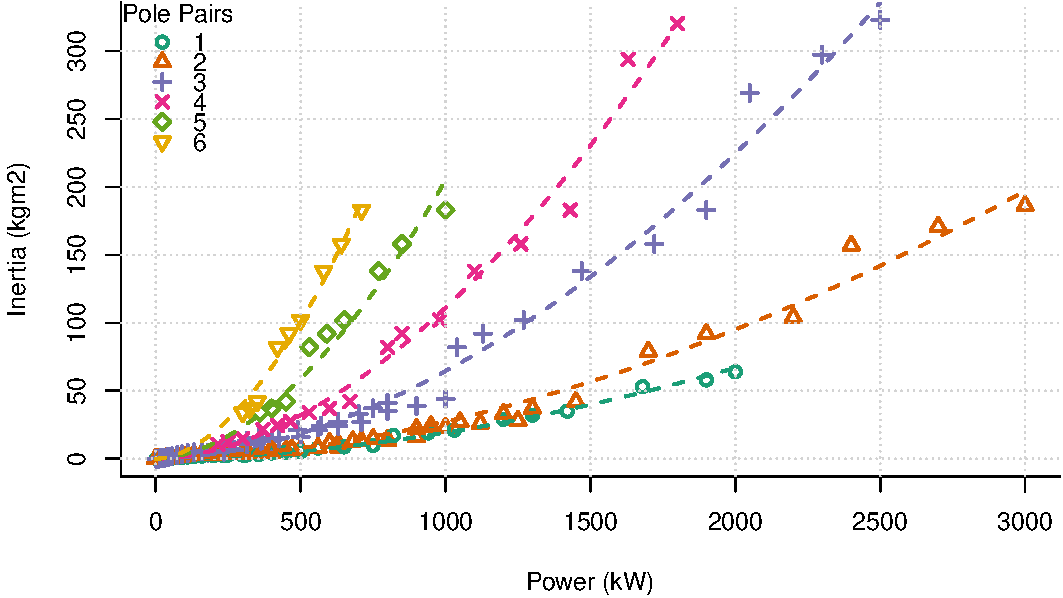
\includegraphics[width=0.5\textwidth]{generator_inertia}}

  \subfloat[Time constant.]{\label{time_constant}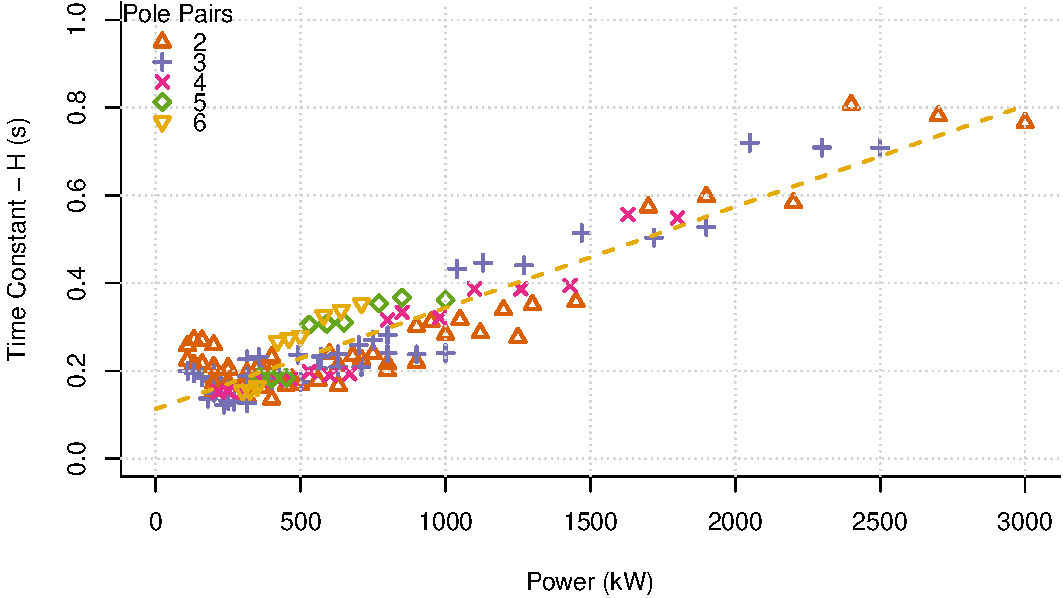
\includegraphics[width=0.5\textwidth]{time_constant}}
    \caption{The rotor inertia and rotor time constant variation as function of pole number and rated power.} 
    \label{inertia_timeconstant}
\end{figure}


\begin{equation}
	H(s)=\frac{\frac{1}{2} J {w_{mech}}^2}{P_{rated}}
	\label{eq:time_constant}
\end{equation}

\begin{equation}
	H(s)=0.00023 \times P_{(kW)} + 0.11335
	\label{eq:time_constant_trend}
\end{equation}

\begin{table*}
  \centering
  \begin{tabular}{lll}
   $N_{pole}$ & Small Machines (<100 kW) & Large Machines (>100 kW) \\
  \hline
2 & $315\times10^{-6}\times {P_{(kW)}}^{1.784}$ & $76\times10^{-6}\times {P_{(kW)}}^{1.8}$ \\
4 & $847\times10^{-6}\times {P_{(kW)}}^{1.68}$ & $109\times10^{-6}\times {P_{(kW)}}^{1.8}$ \\
6 & $4367\times10^{-6}\times {P_{(kW)}}^{1.471}$ & $257\times10^{-6}\times {P_{(kW)}}^{1.8}$ \\
8 &  & $442\times10^{-6}\times {P_{(kW)}}^{1.8}$ \\
10 & & $816\times10^{-6}\times {P_{(kW)}}^{1.8}$ \\
12 & & $1393\times10^{-6}\times {P_{(kW)}}^{1.8}$ \\
\hline
  \end{tabular}
  \caption{Rotor Inertia($kg m^2$) estimation for induction machines as a function of number of poles and rated power.}
  \label{inertia_estimation}
\end{table*}


\subsection{Electrical Parameters} % (fold)
\label{sub:electrical_parameters}

Similar approximations are performed for the electrical parameters of the induction generator.

Refleri kontrol et \cite{Thiringer2001} 

It is easier to represent these parameters in per unit system. The stator resistance variation (in per unit) as a function of the rated power is presented in Fig. \ref{Rs}. It can be seen from the Fig. \ref{Rs_log_plot} that the stator resistance changes linearly in the logarithmic scale. The stator resistance can be estimated as:

\begin{equation}
 	ln(R_s(pu))=-0.3772\;ln (P_{(kW)}) - 2.441
 	\label{eq:Rs}
 \end{equation} 

\begin{figure}[]
  \centering
  \subfloat[Linear Y-axis.]{\label{Rs_plot}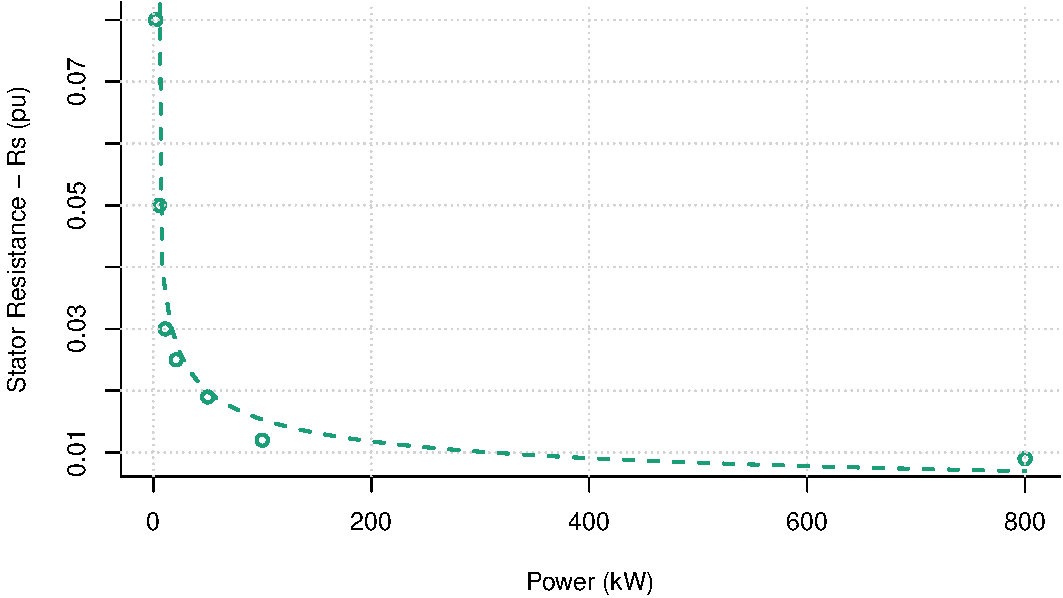
\includegraphics[width=0.5\textwidth]{Rs_plot}}

  \subfloat[Logarithmic Y-axis.]{\label{Rs_log_plot}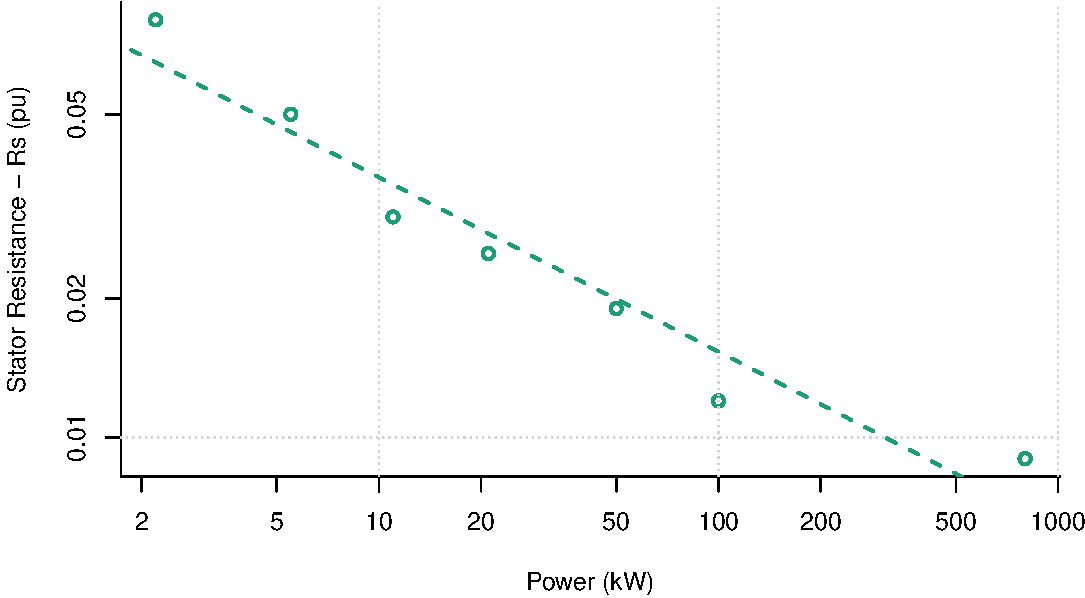
\includegraphics[width=0.5\textwidth]{Rs_log_plot}}
    \caption{Rotor resistance (in per unit) variation as a function of the rated power.} 
    \label{Rs}
\end{figure}

Magnetising inductance ($L_m$) is proportional to the magnetic flux in the machine. The magnetising inductance as a function of the power rating is presented in Fig. \ref{Lm_plot}. Another factor is the leakage inductance, which has a direct effect to the rated power factor of the machine. The leakage inductance as a function of the rated power is presented in Fig. \ref{Lls_plot}. These inductances can be estimated as follows:

\begin{equation}
 	L_m (pu) = 0.158\;ln (P_{(kW)}) + 2.23
 	\label{eq:Lm}
 \end{equation} 

\begin{equation}
 	L_{ls}(pu) = -0.3772 \;ln (P_{(kW)}) - 2.441
 	\label{eq:Lls}
 \end{equation} 


\begin{figure}[]
  \centering
  \subfloat[Mutual inductance, $L_m$.]{\label{Lm_plot}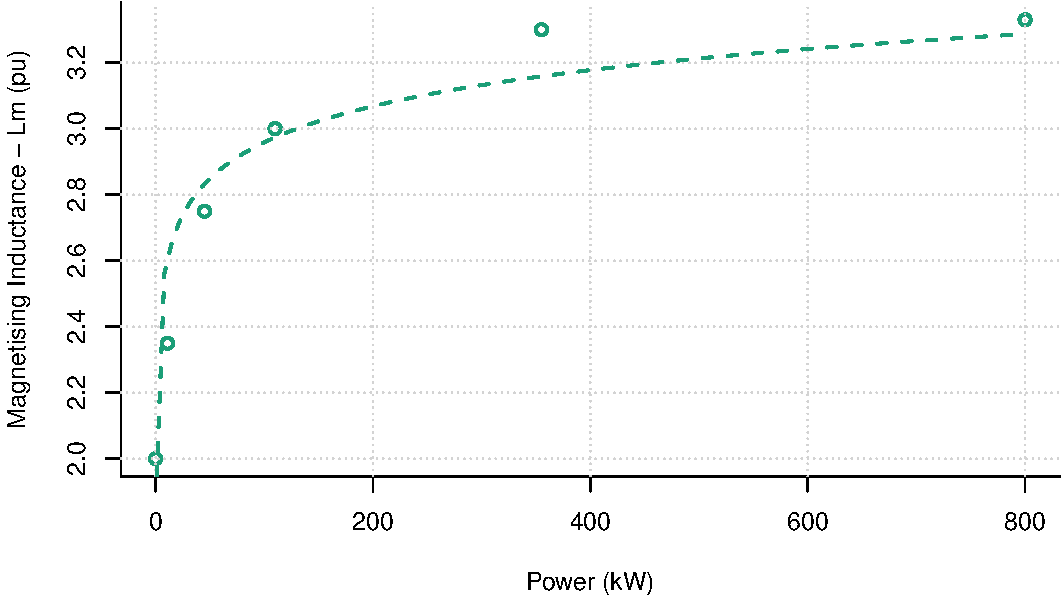
\includegraphics[width=0.5\textwidth]{Lm_plot}}

  \subfloat[Stator leakage inductance, $L_{ls}$.]{\label{Lls_plot}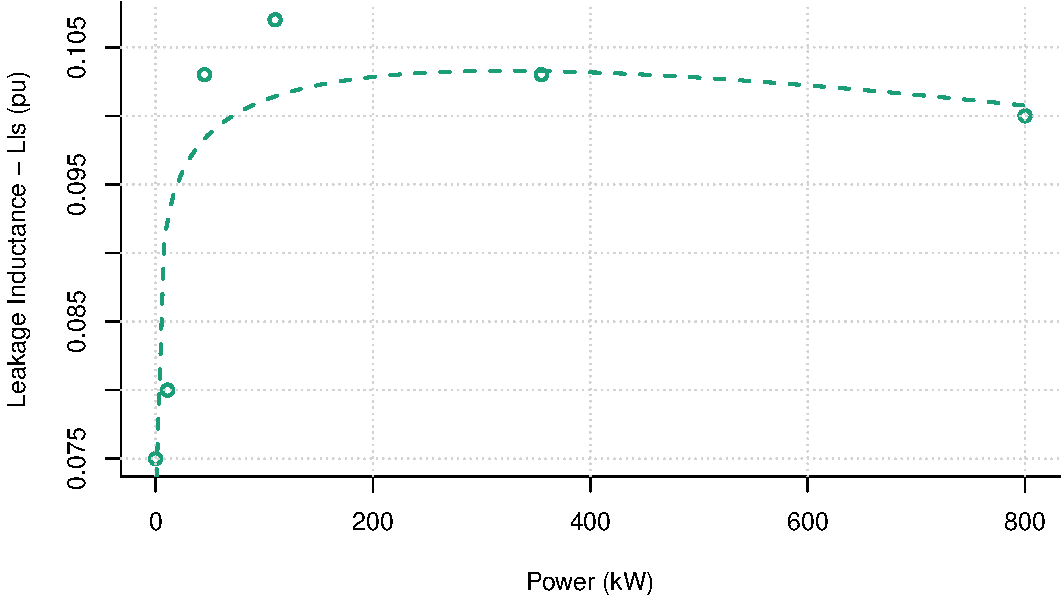
\includegraphics[width=0.5\textwidth]{Lls_plot}}
    \caption{Variation of mutual and stator leakage inductance (in per unit) as a function of the rated power.} 
    \label{inductance_plots}
\end{figure}

% subsection electrical_parameters (end)

\section{Approach}
- Data from two sites (the coast of Norway and Spain) are obtained to get a better representation of the wave and wind energy outputs. These data represent the 10 year measurements for the wind speed and wave height.
- Comprehensive set of Simulink models are developed to model the Wind turbines and Oscillating water columns (OWCs).
- Two different drive trains are used for the wind turbine: doubly fed induction generator coupled to a three stage gearbox and a medium speed permanent magnet generator coupled to a two stage gearbox.
- Well's turbines are used in oscillating water columns, which are connected to induction generators. The speed of the generators are adjusted to maintain maximum aerodynamic efficiency in the Well's turbines.
- The output of the generators are rectified using independent rectifiers and all these rectifiers are connected to a common DC-link to minimize the inverter and step-up transformer cost and to smooth out the power output.
- Simulations with different power ratings are performed and the annual energy generation is recorded in each simulation. These data will be used to find out the optimum generator rating (e.g. maximum energy output and minimun initial cost).
- In the full paper, it is planned to extend the electrical models with a coupled thermal model that will simulate the air-flow and temperature increase in the generators. By this way, it would be possible to utilize the improved thermal performance of a generator in a offshore platform due to increased air circulation and humid environment.

\section{Main Body of Abstract}

Deep water offshore wind and wave energy platforms have larger energy resources compared to onshore equivalents. The MARINA Platform Project, which is a 4.5 year funded EU FP7 project, aims to provide different combined offshore wind and wave energy platforms [1]. One of the challenges in offshore floating platforms is the high installation and operational costs due to challenging environment. The cost of the system can be minimized by optimizing the power rating of the drive-train. 

In this paper, in particular the optimal power rating of the electrical generators will be investigated. This can be achieved in two ways: Firstly, the electrical generators in a wave energy converter operate at partial-loads almost all the time due to the nature of the resource. Thus, the power rating can be reduced without affecting the energy output. Secondly, the electrical generators are subject to increased air circulation with high humidity, which improves the thermal performance significantly [2]. Therefore, they can be over loaded for a short amount of time.

A 5.2 MW wind turbine coupled to ten independent oscillating water columns (OWCs) with Well's turbine are analysed. The rated mechanical energy input for each OWCs is 500 kW. It is possible to choose 500 kW generators, which is the usual practice, however, in this case the capacity factor of the generators would be very low. Alternatively, it is possible to use a smaller power rated generator, but this would reduce the energy harvest as the maximum power is limited. Simulations at different wind-wave conditions (i.e. high wind-low wave, low wind-high wave) are performed for different power rated generators. The measured data series from two sites (off the coast of Norway and Spain) are used the estimate the annual energy harvest of the platform for each power ratings. The main characteristics of the wave and wind resource are presented in Fig. 1-2 and Fig 3-4.

{f1} Probability density distribution of the significant wave height in the coast of Norway.

{f2} Probability density distribution of the wind speed in the coast of Norway.

{f3} Probability density distribution of the significant wave height in the coast of Spain.

{f4} Probability density distribution of the wind speed in the coast of Spain.

Typical power outputs of the wind turbine and one of the OWCs are presented in Fig. 5. Annual energy generation versus the generator power rating is presented in Fig. 6. The figure shows that if the generator rating is decreased by 60 \% (to 200 kW), the energy harvest just reduces by 15 \%.  In this simulation, the increase in the thermal performance of the machine is not taken into account yet. In the full paper, it is planned to couple the electrical model with a thermal model that can simulate the airflow around the generator. In this way, it would be possible to overload the generator  for a short amount time, and this will make if possible to get the same energy output from a smaller generator. Furthermore, it is planned to include power smoothing between OWCs (such as common DC-link), which will help to reduce the size of other components such as switches and cables.

\section{Conclusion}

This paper focuses on the optimum sizing of the electrical generators in a combined wind and wave energy platform. The floating platform has a single wind turbine and ten independent oscillating water columns. Simulink models are developed to simulate the energy output from the wind turbine and OWCs. The OWCs are connected to a common DC-link with separate controlled rectifiers. The wind turbines has separate inverters and step-up transformers.

{f5} Typical power output from the wind turbine and one of the oscilating water columns.

{f6} The annual energy generation versus the generator power rating (for a single oscilation water column).

Time series data from the coast of Norway and Spain are used to estimate the energy harvest for different generator ratings. The aim is to minimize the initial cost of the drive train without affecting the electricity generation income. The preliminary results show that the generator size can be reduced by 60% with a 15 % decrease in the wave energy output. It is also planned to include a coupled thermal model in the full paper, which simulate the operating conditions in a offshore platform more realistically.

{f5} Typical power output from the wind turbine and one of the oscilating water columns.

{f6} The annual energy generation versus the generator power rating (for a single oscilation water column).

Time series data from the coast of Norway and Spain are used to estimate the energy harvest for different generator ratings. The aim is to minimize the initial cost of the drive train without affecting the electricity generation income. The preliminary results show that the generator size can be reduced by 60\% with a 15\% decrease in the wave energy output. It is also planned to include a coupled thermal model in the full paper, which simulate the operating conditions in a offshore platform more realistically.


\section{Learning Objectives} % (fold)
\label{sec:learning_objectives}

The paper presents Matlab/Simulink models of a wind turbine coupled to oscillating water columns. The thermal models of the generators will be also presented. These models will be shared as open-source, which will enable delegated to use the models for their own systems.

% section learning_objectives (end)

\section{References from first} % (fold)
\label{sec:references_from_first}
[1] Barrios, I. Martinez, J. Murphy, K. Lynch, and C. Lopez Pavon. "Methodology for assessing multiple combined wind and ocean energy technologies as part of the EU FP7 MARINA Platform Project." ICOE 2012 Proceedings, Dublin, Ireland (2012).
[2] Hodgins, Neil. "High speed electrical power takeoff for oscillating water columns." ,University of Edinburgh PhD Dissertation, (2010).
% section references_from_first (end)


\section{Methods}

Maecenas sed ultricies felis. Sed imperdiet dictum arcu a egestas. 
\begin{compactitem}
\item Donec dolor arcu, rutrum id molestie in, viverra sed diam
\item Curabitur feugiat
\item turpis sed auctor facilisis
\item arcu eros accumsan lorem, at posuere mi diam sit amet tortor
\item Fusce fermentum, mi sit amet euismod rutrum
\item sem lorem molestie diam, iaculis aliquet sapien tortor non nisi
\item Pellentesque bibendum pretium aliquet
\end{compactitem}
\lipsum[4] % Dummy text

%------------------------------------------------

\section{Results}

\begin{table}[H]
\caption{Example table}
\centering
\begin{tabular}{llr}
\toprule
\multicolumn{2}{c}{Name} \\
\cmidrule(r){1-2}
First name & Last Name & Grade \\
\midrule
John & Doe & $7.5$ \\
Richard & Miles & $2$ \\
\bottomrule
\end{tabular}
\end{table}

\lipsum[5] % Dummy text

\begin{equation}
\label{eq:emc}
e = mc^2
\end{equation}

\lipsum[6] % Dummy text


\section*{Acknowledgement} % (fold)
\label{sec:acknowledgement}

The authors gratefully acknowledge the financial support
from the EU FP7 MARINA Platform project, grant agreement no. FP7-241402.
% section acknowledgement (end)
%------------------------------------------------

\section{Discussion}

\subsection{Subsection One}

\lipsum[7] % Dummy text

\subsection{Subsection Two}

\lipsum[8] % Dummy text

%----------------------------------------------------------------------------------------
%	REFERENCE LIST
%----------------------------------------------------------------------------------------

\begin{thebibliography}{99} % Bibliography - this is intentionally simple in this template

\bibitem[Figueredo and Wolf, 2009]{Figueredo:2009dg}
Figueredo, A.~J. and Wolf, P. S.~A. (2009).
\newblock Assortative pairing and life history strategy - a cross-cultural
  study.
\newblock {\em Human Nature}, 20:317--330.
 
\end{thebibliography}

%----------------------------------------------------------------------------------------

%\end{multicols}

\end{document}
